% !TEX root = ../md2-user-handbook.tex
% !TeX spellcheck = en_US
% !TeX program = xelatex
\subsection{Creating a Project}
\begin{enumerate}
\item  Initialize a new project by navigating to \lstinline[language=Simple]|File > New > Project...|. There, choose \lstinline[language=Simple]|Other > MD2 Project| and click \lstinline|Next|.
\item Choose a project name that does not contain whitespace or other non-alphanumerical characters. If necessary, choose a location different from the proposed default.
\item After clicking on \lstinline|Finish|, a default project structure is generated which you can extend as you need.
\end{enumerate}

The new project contains the following folders:

\begin{itemize}
\item \lstinline[language=Simple]|src/| contains the \MD models of your application and is initialized with a simple default model.
\item \lstinline[language=Simple]|resources/| contains resources that the generator will copy into the generated applications.
\item \lstinline[language=Simple]|src-gen/| contains all artifacts that the generator derives from your model. This folder will contain multiple subfolder for different platforms. For example, there might be a folder for the backend and for \mapapps. Note, that everything in this directory will be overwritten when the generator is run.
\end{itemize}

\subsection{Developing a Single App} 
\label{subsec:SingleAppDev}
This section describes how an application can be developed based on the current (March 2015) state of the \MD DSL. At its core, \MD is structured according to the MVC-pattern. MVC stands for Model-View-Controller and ensures the principle of single responsibility for these classes. In order to enable the modelling and generation of worklows within across apps in \MD, this architecture was extended to include an additional layer, the workflow layer (cf. \Cref{fig:MD2Arch}).

%\begin{figure}[htb!]
%\centering
%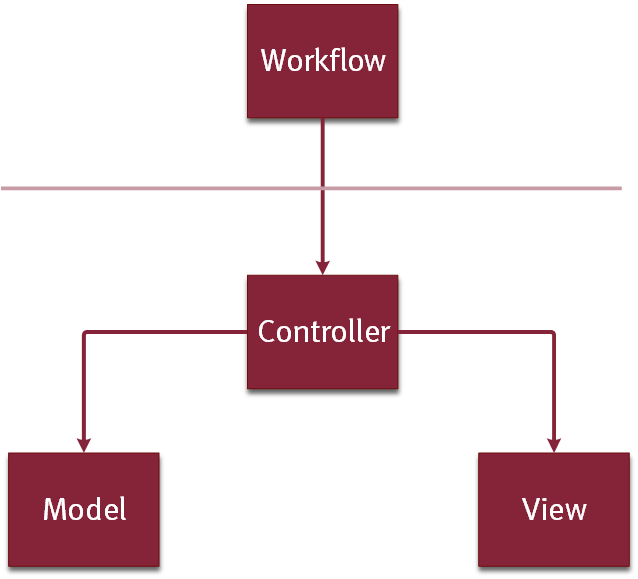
\includegraphics[width = 0.4\linewidth]{Fig/MD2Arch.png}
%\caption{Architecture of \MD Models}
%\label{fig:MD2Arch}
%\end{figure}

\begin{figure}[htb!]
\centering
\begin{tikzpicture}[redbox/.style = {rectangle, fill=ercisred, text =white, text width=5em, minimum height = 3em, text centered, drop shadow}, >=stealth]
	\node[redbox] (wf) {Workflow};
	\node[redbox, below = of wf] (ctrl) {Controller};
	\node[redbox, below left = of ctrl] (model) {Model};
	\node[redbox, below right = of ctrl] (view) {View};
	\draw[->, thick, ercisred] (wf) -- (ctrl);
	\draw[->, thick, ercisred] (ctrl) -| (model);
	\draw[->, thick, ercisred] (ctrl) -| (view);
	\draw[gray!50!ercisred, thick, dashed] ($ (wf.south west) + (-1.5cm,-0.5cm) $) -- ($ (wf.south east) + (1.5, -0.5cm) $);
\end{tikzpicture}
\caption{Architecture of \MD models}
\label{fig:MD2Arch}
\end{figure}

All components in \MD are organized in a package structure that corresponds to the aforementioned structure. Documents have to be placed in these packages (views, models, controllers or workflow). For example, all view files are expected to be in the package \lstinline[language=Simple]|any.project.package.views|. In every \MD file the package has to be defined as follows:
\begin{lstlisting}
package PACKAGE_NAME
\end{lstlisting}
The package name has to be a fully qualified name that reflects the actual folder structure.

\subsubsection{Workflow} 
\label{subsubsec:Workflow}
% !TEX root = ../md2-user-handbook.tex
% !TeX spellcheck = en_US
% !TeX program = xelatex

The workflow layer provides abstraction on top of the controller layer. It allows to specify the general course of action of one or more apps using a few simple and easily understandable model language constructs. Furthermore, this abstract workflow representation is intended to serve as a basis for communication with customers, e.g. for requirements engineering and collaborative app development through rapid prototyping.

Workflows are specified as a (possibly cyclic) directed graph of workflow elements in the workflow file of an \MD model. Workflow elements represent encapsulated functionality which needs to be further specified in the controller layer. The workflow layer merely references the workflow elements from the controller layer to define their interaction.

Workflow elements are linked to each other via events. For each workflow element one or more events can be specified that can be fired. However, at runtime a workflow element can fire only one of these events, i.\,e. a parallel processing of the workflow is not intended. Similar to the workflow elements, workflow events in the workflow layer are references to workflow events that are created in the respective controller.

In addition to the events that can be fired, the workflow element also specifies which workflow element is to be started in response to a fired event using the keyword {\lstinline!start!}. Moreover, when an event is fired, not only workflow elements can be started but the workflow can be terminated by using the \lstinline!end workflow! keyword.
A workflow element in the workflow layer typically looks as shown in Listing \ref{lst:wfe}.

\begin{lstlisting}[language=MD2, label=lst:wfe, caption=Workflow Elements in the Workflow Layer]
 WorkflowElement <NameOfWorkflowElement>
 	fires <NameOfEventOne> {
		start <NameOfSubsequentWfeOne>
	}
	fires <NameOfEventTwo> {
		end workflow
	}
\end{lstlisting}

After defining the sequence of workflow elements, the workflow also requires the specification of an app that executes the workflow elements. As shown in Listing \ref{lst:app}, an app consists of its ID, a list of workflow elements that are used in the app and a name that is to be used as the app title. In the scenario where only a single app is modeled, all workflow elements can be listed in the app. However, it is also possible to have unused workflow elements.

\begin{lstlisting}[language=MD2, label=lst:app, caption=App Definition in \MD]
App <AppID> {
	WorkflowElements {
		<WorkflowElementOne>,
		<WorkflowElementTwo> (startable: STRING),
		<WorkflowElementThree> 
	}
	appName STRING
}
\end{lstlisting}

A workflow has one or more entry points, i.\,e. startable workflow elements. These are marked as {\lstinline!startable!} in the app specification. During code generation this will result in a button on the app's start screen that starts the corresponding workflow element. In addition, an alias needs to be provided which is used as label or description for the button.

Finally, the complete workflow specification for one app will be structured as shown in Listing \ref{lst:workflow}. Note that \MD does not differentiate between different workflows. However, it is possible to implicitly create multiple workflows by using two or more startable workflow elements that start independent, disjunct sequences of workflow elements.

\begin{lstlisting}[language=MD2, label=lst:workflow, caption=Workflow Definition in \MD]
package <ProjectName>.workflows

WorkflowElement <WorkflowElementOne>
[...]
WorkflowElement <WorkflowElementTwo>
[...]
WorkflowElement <WorkflowElementThree>
[...]

App <AppID> {
	[...]
}
\end{lstlisting}

\subsubsection{Model} 
\label{subsubsec:Model}
% !TeX spellcheck = en_US
% !TeX program = xelatex
% !TeX root = ../md2-user-handbook.tex

In the model layer the structure of data objects is being described. As model elements Entities and Enums are supported.
\paragraph{Entity}
An entity is indicated by the keyword {\lstinline!entity!} followed by an arbitrary name that identifies it.
\begin{lstlisting}
entity NAME {
	<attribute1 ... attribute n>
}
\end{lstlisting}
Each entity may contain an arbitrary number of attributes of the form
\begin{lstlisting}
ATTRIBUTE_NAME: <datatype>[] (<parameters>) {
	name STRING
	description STRING
}
\end{lstlisting}
The optional square brackets [] indicate a one-to-many relationship. That means that the corresponding object may hold an arbitrary number of values of the given datatype.
Supported complex data types are:
\begin{itemize}
\item{Entity}
\item{Enum}
\end{itemize}
Supported simple data types are:

\begin{itemize}
\item{\lstinline!integer! -- integer}
\item{\lstinline!float! -- float of the form \#.\#}
\item{\lstinline!boolean! -- boolean}
\item{\lstinline!string! -- a string that is embraced by single quotes (') or double quotes (")}
\item{\lstinline!date! -- a date is a string that conforms the following format: \lstinline!YYYY-MM-DD!}
\item{\lstinline!time! -- a time is a string that conforms the following format: \lstinline!hh:mm:ss[(+|-)hh[:mm]]!}
\item{\lstinline!datetime! -- a date time is a string that conforms the following format: \lstinline!YYYY-MM-DDThh:mm:ss [(+|-)hh[:mm]]!}
\item{\lstinline!file! -- a file to be uploaded and stored in an entity field}
\end{itemize}

Parameters are optional and will be transformed into implicit validators during the generation process. They have to be specified as a comma-separated list. On default each specified attribute is mandatory. To allow null values the parameter optional can be set. Further supported parameters depend on the used data type and are explained as follows:

\begin{itemize}
\item \lstinline!integer! supports
\subitem \lstinline!max INTEGER! – maximum allowed value of the attribute
\subitem \lstinline!min INTEGER! – minimum allowed value of the attribute
\item \lstinline!float! supports
\subitem \lstinline!max FLOAT! – maximum allowed value of the attribute
\subitem \lstinline!min FLOAT! – minimum allowed value of the attribute
\item \lstinline!string! supports
\subitem \lstinline!maxLength INTEGER! – maximal length of the string value
\subitem \lstinline!minLength INTEGER! – minimal length of the string value
\end{itemize}

Optionally, attributes can be annotated with a name and a description which are used for the labels and the tooltips in the auto-generation of views. If a tooltip is annotated a question mark will be shown next to the generated input field. If no name is annotated, a standard text for the label will be derived from the attribute's name by transforming the camel case name to natural language. E.g. the implicit label text of the attribute firstName is \enquote{First name}.

Exemplary entity that represents a person:
\begin{lstlisting}
entity Person {
	name: string
	birthdate: date {
		name: "Date of Birth"
		description: "The exact day of birth of this person."
	}
	salary: float (optional, min 8.50, max 1000)
	addresses: Address[]
}
\end{lstlisting}

\paragraph{Enum}
An enumeration is indicated by the keyword \lstinline!enum! followed by an arbitrary name that identifies it. Each enum may contain an arbitrary number of comma-separated strings. Other data types are not supported.
Exemplary enum element to specify weekdays:
\begin{lstlisting}
enum Weekday {
	"Mon", "Tue", "Wed", "Thu", "Fri", "Sat", "Sun"
}
\end{lstlisting}

\subsubsection{View} 
\label{subsubsec:View}
% !TeX spellcheck = en_US
% !TeX program = xelatex
% !TeX root = ../md2-user-handbook.tex

View elements are either ContentElements or ContainerElements that can contain other content or container elements. Furthermore, basic styles for some content elements can be defined.

\paragraph{Container Elements}

\textit{Grid layout panes} align all containing elements in a grid. Elements can either be containers or content elements. The grid is populated row-by-row beginning in the top-leftmost cell.

\begin{lstlisting}
GridLayoutPane NAME (<parameters>) {
	<Container | Content | [Container] | [Content]>
	<Container | Content | [Container] | [Content]><...>
}
\end{lstlisting}

For each grid layout at least the number of rows or the number of columns has to be specified. If only one of these parameters is given, the other one is automatically calculated by \MD during the generation process. In case that both parameters are specified and there are too few cells, all elements that do not fit in the layout will be discarded. The following comma-separated parameters are supported:
\begin{itemize}
\item \lstinline!columns INTEGER! -- the number of columns of the grid
\item \lstinline!rows INTEGER! -- the number of rows of the grid
\item \lstinline!tabIcon PATH! -- if the layout is a direct child of a TabbedPane, an icon can be specified that is displayed on the corresponding tab. See section on TabbedPanes for more details.
\item \lstinline!tabTitle STRING! -- if the layout is a direct child of a TabbedPane, a text can be specified that is displayed on the corresponding tab. See section on TabbedPanes for more details.
\end{itemize}

A \textit{flow layout pane} arranges elements (containers or content elements) either horizontally or vertically. By default all elements are arranged vertically in a left-to-right flow.
\begin{lstlisting}
FlowLayoutPane NAME (<parameters>) {
	<Container | Content | [Container] | [Content]>
	<Container | Content | [Container] | [Content]>
	<...>
}
\end{lstlisting}
The following comma-separated parameters are supported:
\begin{itemize}
\item \lstinline!vertical! or \lstinline!horizontal! (default) -- flow direction
\item \lstinline!tabIcon PATH! -- if the layout is a direct child of a TabbedPane (which are described subsequently), an icon can be specified that is displayed on the corresponding tab.
\item \lstinline!tabTitle STRING! -- if the layout is a direct child of a TabbedPane, a text can be specified that is displayed on the corresponding tab.
\end{itemize}

A \textit{tabbed pane} is a special container element that can only contain container elements. Each contained container will be generated as a separate tab. Due to restrictions on the target platforms, tabbed panes can only be root panes, but not a child of another container element. By default the title of each tab equals the name of the contained containers. By using the tabTitle and tabIcon parameters the appearance of the tabs can be customized.
\begin{lstlisting}
TabbedPane NAME {
	<Container | [Container]>
	<Container | [Container]>
	<...>
}
\end{lstlisting}

\paragraph{Content Elements}
\textit{Input elements} can be used to manipulate model data via mappings (see Section \ref{subsubsec:Controller}). At the moment BooleanInputs, TextInputs, IntegerInputs, NumberInputs, TimeInputs, DateInputs, DateTimeInputs, OptionInputs and FileUploads are supported. All input elements support the optional attributes \lstinline!label!, \lstinline!tooltip!, \lstinline!type!, \lstinline!disabled!, \lstinline!default! and \lstinline!width!. \lstinline!type! allows to specify the type of the field. \lstinline!disabled! provides a boolean for whether an input field is enabled or disabled. Default values can be set using \lstinline!default! and the width using \lstinline!width!.

\textit{TextInput} fields can be used for freetext as well as date and time inputs.
\begin{lstlisting}
TextInput NAME { 
	label STRING
	tooltip STRING
	type <TextInputType>
	disabled <true|false>
	default STRING)
	width <width>
}
\end{lstlisting}

\textit{OptionInputs} are used to represent enumeration fields in the model. In addition to the aforementioned attributes, OptionInputs support the optional \lstinline!options! attribute. This can be used to populate the input with the string values of the specified enum. If options are not given, the displayed options depend on the enum type of the attribute that has been mapped on the input field (see Section \ref{subsubsec:Controller}).
\begin{lstlisting}
OptionInput NAME { 
	label STRING
	tooltip STRING
	type <OptionInputType>
	disabled <true|false>
	default STRING
	width <width>
	options <enum>
}
\end{lstlisting}

\textit{Labels} allow the modeler to present text to the user. Often they are used to denote input elements. For the label definition there exist the following default definition
\begin{lstlisting}
Label NAME {
	text STRING
	style <[style] | style>
}
\end{lstlisting}
as well as this shorthand definition
\begin{lstlisting}
Label NAME (STRING){
	style <[style] | style>
}.
\end{lstlisting}

The text can either be annotated as an explicit text attribute or noted in parentheses directly after the label definition. The optional style can either be noted directly, or by referencing an existing style definition (styles are described later in this section).

\textit{Tooltips} allow the modeler to provide the user with additional information. For the tooltip definition there exists the following default definition
\begin{lstlisting}
Tooltip NAME {
	text STRING
}
\end{lstlisting}

as well as this shorthand definition that allows to note the help text in parentheses directly after the label definition
\begin{lstlisting}
Tooltip NAME (STRING).
\end{lstlisting}

\textit{Buttons} provide the user the possibility to call actions that have been bound on events of the Button. For the button definition there exists the following default definition
\begin{lstlisting}
Button NAME {
	text STRING
}
\end{lstlisting}
as well as this shorthand definition that allows to specify the text in parentheses directly after the button definition
\begin{lstlisting}
Button NAME (STRING).
\end{lstlisting}


For the \textit{image} exists the following default definition
\begin{lstlisting}
Image NAME {
	src PATH
	height INT
	width INT
}
\end{lstlisting}
as well as this shorthand definition that allows to specify the image path in parentheses directly after the image name
\begin{lstlisting}
Image NAME (PATH) {
	height INT
	width INT
}.
\end{lstlisting}
Images support the following attributes:
\begin{itemize}
\item \lstinline!src! -- Specifies the source path where the image is located. The path has to be relative to the directory /resources/images in the folder of the \MD project
\item \lstinline!height! (optional) -- Height of the image in pixels
\item \lstinline!width! (optional) -- Width of the image in pixels
\end{itemize}


While the \lstinline!Image! construct can only be used to display images that have a fixed URI, the \textit{UploadedImageOutput} can be used to display images that are stored in a field of an entity and were uploaded before. \lstinline!UploadedImageOutput! features the same attributes as \lstinline!Image! and is specified as follows.

\begin{lstlisting}
UploadedImageOutput NAME {
	height INT
	width INT
}
\end{lstlisting}

\textit{FileUpload} is an input element for files. Using this construct, a button having the specified attributes and allowing for uploading a file is displayed on the respective UI form. \lstinline!FileUpload! can be specified using the following attributes.

\begin{lstlisting}
FileUpload NAME {
	label STRING
	text STRING
	tooltip STRING		
	style <[style] | style>
	width INT%
}	
\end{lstlisting}

To be able to display an uploaded image using the \lstinline!UploadedImageOutput! construct, it is necessary to map the respective view elements to the corresponding entity fields in the controller as it is applicable for all other view content elements. 

A \textit{Spacer} is used in a \lstinline!GridLayoutPane! to mark an empty cell or in a \lstinline!FlowLayoutPane! to occupy some space.
Using an optional additional parameter the actual number of generated spacers, \ie the number of occupied cells in  a \lstinline!GridLayoutPane!, can be specified.
\begin{lstlisting}
Spacer (INT)
\end{lstlisting}

The \textit{AutoGenerator} is used to automatically generate view elements to display all attributes of a related entity and the corresponding mappings of the view elements to a content provider. It is possible to either exclude attributes using the \lstinline!exclude! keyword or to provide a positive list of attributes using the keyword \lstinline!only!.
\begin{lstlisting}
AutoGenerator NAME {
	contentProvider [ContentProvider] (exclude|only [Attribute])
}
\end{lstlisting}

In case of one-to-many relationships for attributes (annotated with []) or a content provider, it has to be defined which of the elements should be displayed in the auto-generated fields. The \textit{EntitySelector} allows the user to select an element from a list of elements. The attribute \lstinline!textProposition! defines which content provider stores the list and which attribute of the elements shall be displayed to the user to allow him to find the desired element.
\begin{lstlisting}
EntitySelector NAME {
	textProposition [ContentProvider.Attribute]
}
\end{lstlisting}

\textit{Styles} can be annotated to several view elements such as labels and buttons to influence their design. They can either be defined globally as a root element in the view and then be referenced, or annotated directly to the appropriate elements.
\begin{lstlisting}
style NAME {
	color <color>
	fontSize INT
	textStyle <textstyle>
}
\end{lstlisting}

The following optional style attributes are supported. If an attribute is not set, the standard setting is used for each platform.
\begin{itemize}
\item \lstinline!color <color>! (optional) -- specifies the color of the element as a named color or a six or eight digit hex color (with alpha channel)
\item \lstinline!fontSize INT! (optional) -- specifies the font size
\item \lstinline!textStyle <textstyle>! (optional) -- the text style can be \lstinline!normal! or \lstinline!italic!, \lstinline!bold! or a combination of both.
\end{itemize}

Sixteen default web colors are available as named colors: \lstinline!aqua, black, blue, fuchsia, gray, green, lime, maroon, navy, olive, purple, red, silver, teal, white, yellow!.

Elements can not only be defined at the place they should be used, but there is also a mechanism to define an element once and \textit{reuse} it several times. Instead of defining a new element, another element can be referenced -- internally this leads to a copy of the actual element during the preprocessing. However, names have to be unique so that each element could only be referenced once. To avoid those name clashes a renaming mechanism had been implemented that allows to set new names for the actual copied element.
\begin{lstlisting}
Element -> NAME
\end{lstlisting}


\subsubsection{Controller} 
\label{subsubsec:Controller}
% !TeX spellcheck = en_US
% !TeX program = xelatex
% !TeX root = ../md2-user-handbook.tex


\subsection{Deploying a Single App}
\label{subsec:SingleAppDep}

\subsubsection{Backend} 
\label{subsubsec:Backend}

The following steps will start the GlassFish server that is used to deploy the backend.
Note, that in order to access the server you might need to grant additional privileges in the configuration of your firewall.d.

\begin{enumerate}
\item Within the GlassFish installation directory, navigate to \lstinline[language=Simple]|glassfish/bin/|.
\item Run the \lstinline[language=Simple]|asadmin| utility (Windows: Double-click on \lstinline[language=Simple]|asadmin.bat|, Linux/OS X: Open a terminal in that directory and run \lstinline[language=Simple]|./asadmin|).
\item In the GlassFish administration utility, type \lstinline[language=Simple]|start-database| to start the Derby database for the backend. In a Unix environment, you can combine both steps by running\\ \lstinline[language=Simple]|./asadmin start-database|.
\item Start Eclipse and import the generated project \lstinline[language=Simple]|<PROJECT_NAME>.backend| by choosing \enquote{General} $\rightarrow$ \enquote{Existing Projects into Workspace} in the import wizard.
\item In the Project Explorer tab, right-click the project in Eclipse, choose \enquote{Properties}, and navigate to \enquote{Targeted Runtime}.
\item Deselect all runtimes and click \enquote{Apply}.
\item Select the item \enquote{GlassFish 4.0} and click \enquote{Apply}.
\item Correct JRE-related build path problems, if any, by resorting to the default JRE.
\item Confirm by clicking \enquote{OK}.
\item In the Servers tab, right-click the \enquote{GlassFish 4.0} entry, and choose \enquote{Add/Remove}.
\item Add the backend project to the server.
\item Start the server.
\end{enumerate}


\subsubsection{\mapapps} 
\label{subsubsec:mapapps}

You have two options to deploy a \mapapps app in your NetBeans development environment:
\begin{itemize}
\item Copy it into the \lstinline[language=Simple]|src/main/js/app/| directory of the project, or
\item use a symbolic link to reference apps from another location (see \Cref{subsec:link-apps}).
\end{itemize} 

An benefit of the second variant is that newly generated code, that results from changes to your model, will automatically be available in your \mapapps development environment. If the server is running, the code will also be deployed to the server automatically.
